\section{Introduction}

\subsection{Longest Common Subsequence}
\begin{frame}
    \frametitle{Longest Common Subsequence}
    %\setlength\itemsep{1em}
    Given two strings $X = x_1 \; x_2 \cdots x_n$ and $Y = y_1 \; y_2 \cdots y_m$.
    \begin{definition}
    	Subsequence $S = s_1 \; s_2 \cdots s_r$ of $X$, we define a 
    	\emph{correspondence sequence} of $X$ and $S$, $C(X, S) = c_1 \; c_2 \cdots c_r$ 
    	to be a strictly increasing sequence of integers such that 
    	$s_i = x_{c_i}$ $1 \le i \le r$
	\end{definition}
	\begin{definition}
		A common subsequence $S$ of $X$ and $Y$, if there exists correspondence sequence
		$C(X, S)$ and $C(Y, S)$.
	\end{definition}
\end{frame}

\subsection{Constrained LCS}
\begin{frame}
    \frametitle{Constrained Longest Common Subsequence}
    \begin{itemize}
    	\item Fixed Gapped LCS with respect to a given integer $K$
    		$$c_i - c_{i-1} \le K+1$$
    	\item Elastic Gapped LCS with respect to given integers $K_1$ and $K_2$
    		$$K_1 < c_i - c_{i-1} \le K_2 + 1$$
    \end{itemize}
\end{frame}

\begin{frame}
    \frametitle{Constrained Longest Common Subsequence}
    \begin{itemize}
        \item Rigid Fixed Gapped LCS
            $$C(X, S)[i] - C(X, S)[i-1] = C(Y, S)[i] - C(Y, S)[i-1]$$
        \item Variable Gapped LCS
            $$C(X, S)[i] - C(X, S)[i-1] \le G_{X}[c_i]$$
            $$C(Y, S)[i] - C(Y, S)[i-1] \le G_{Y}[c_i]$$
    \end{itemize}
\end{frame}

\begin{frame}
    \frametitle{Serial Algorithm Analysis}
    \begin{center}
        \begin{tabular}{l l l l}
            \hline
            Problem & Time  & Space     & Data Structure \\ \hline
            FIG     & $n^2$                 & $n^2$ & Monotone queue \\ \hline
            ELAG    & $n^2 + \mathcal{R} \log \log n$   & $\max(\mathcal{R}, n)$ & van Emde Boas\\ \hline
            RLCS    & $n^2$                 & $n^2$ & \\ \hline
            RIFIG   & $n^2$                 & $n^2$ & \\ \hline
            VG      & $n^2 \; \alpha(n)$    & $n^2$     & Disjoint-set\\ \hline
        \end{tabular}
    \end{center}
\end{frame}

\begin{frame}
    \frametitle{VGLCS Example}
    \begin{figure}
        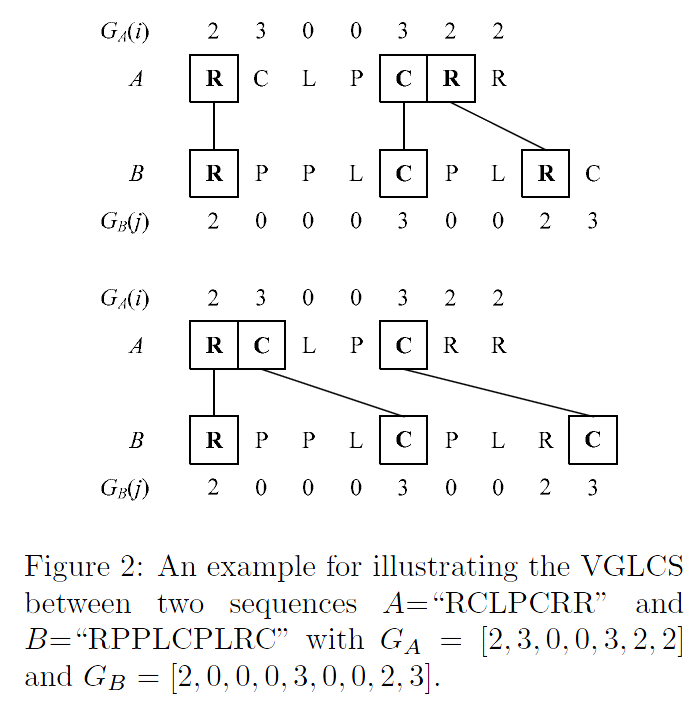
\includegraphics[scale=0.3]{figure/fig-VGLCS-ex.png}
    \end{figure}
\end{frame}

\subsection{Serial VGLCS Algorithm}
\begin{frame}
    \frametitle{Serial VGLCS Algorithm}
    \begin{figure}
        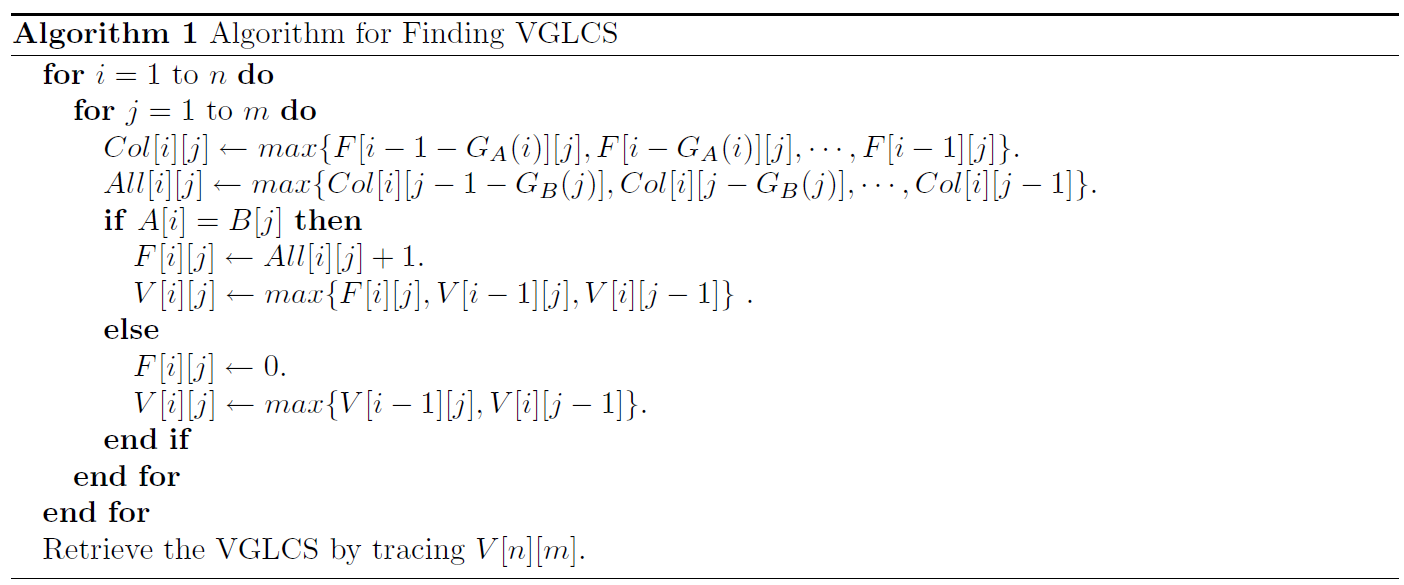
\includegraphics[scale=0.3]{figure/fig-VGLCS-algo.png}
    \end{figure}
\end{frame}

\subsection{Contributions (TODO)}
\begin{frame}
    \frametitle{Contributions}
\end{frame}
